% !TeX root = ../main.tex

% Copyright (c) 2022 myl7
% SPDX-License-Identifier: CC-BY-NC-ND-4.0

\chapter{设计方案}

\section{基础架构}

xdptun 这套 UDP over TCP 方案的最终分发产物为两份 eBPF 二进制文件,分别处理入方向和出方向的流量。
其中入方向的 eBPF 文件挂载到 Linux 中的 XDP 入方向挂载点,而出方向的 eBPF 文件挂载到 Linux 中的 TC 出方向挂载点。
入方向上,数据帧在被网卡设备接受后,根据 XDP 挂载模式,会在网卡中直接触发 XDP 入方向挂载点上程序的处理,或是在网卡将数据帧发送给 Linux 内核后,于 Linux 内核网络栈最前端、在 SKB 分配前或是分配后触发同样的处理程序。
经过处理后的数据帧会重入 Linux 内核网络栈,正常地经由 Linux 内核网络栈中入方向各部件处理后,再递送给用户态监听的程序。
而在出方向上,网络数据在被用户态程序发送给 Linux 内核网络栈后,首先经过 Linux 内核网络栈中出方向各部件处理,最后以数据帧的形式在 Linux 内核网络栈末尾触发 TC 出方向挂载点上程序的处理。
经过处理后的数据帧被递送给网卡设备,再被发送到网络之中。
概括性的流程图如图~\ref{fig:flow} 所示。

\begin{figure}[h]
  \centering
  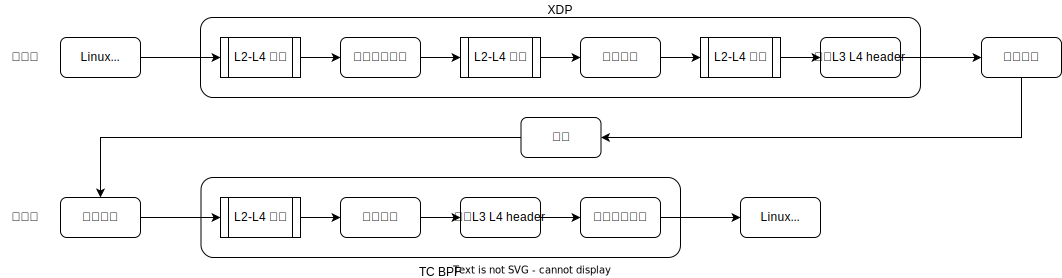
\includegraphics[width=1\textwidth]{xdptun-flow.drawio.pdf}
  \caption{出入方向数据帧处理流程}
  \label{fig:flow}
  \note{图中 L2、L3、L4 分别为链路层、网络层、传输层的缩写}
\end{figure}

\section{出方向处理}

\subsection{流量过滤}

出方向处理程序中,首先进行的是流量过滤,从而保证程序只捕捉需要处理的特殊流量而将其他无关流量原样递送给网卡设备。
特殊流量的匹配方式允许用户利用链路层到传输层的头部各字段进行自定义,但我们提供的模版是通过传输层目标地址和目标端口进行匹配的,能满足大部分需求。
整个匹配过程中,我们首先获取到数据帧的首指针和尾指针,然后从链路层到传输层、借助 Linux 网络相关头文件中各协议头部的 \texttt{struct} 结构来完成解析。
具体而言,从链路层到传输层,我们保证匹配的数据帧对应地是 ETH(Ethernet)、IPv4、UDP 协议。
此过程中,一方面可以校验帧中各头部合法且未导致边界外的内存访问,另一方面也能获取到链路层至传输层各头部的结构、从而支持用户的自定义过滤和后续的帧数据处理。
这里对于内存访问边界的校验同样会保证程序在编译后可以通过 BPF 校验器,从而能被成功加载入 Linux 内核中。
整个匹配完成后,程序就获得了链路层到传输层头部各字段的访问方式,并提取出了需要处理的特殊数据帧,进而可以进行下一阶段的帧数据修改。

\subsection{扩展帧尾空间}

在本方案中,将 UDP 流量伪装为 TCP 流量的核心思路是将 UDP 头部转化为 TCP 头部。
比较 UDP 头部和 TCP 头部,两者前 4 字节的源端口、目标端口两字段位置是相同的,因而不需要处理。
而后续的字段中,UDP 头部上剩余的 4 字节是包长和校验和,对应占据了 TCP 头部中序列号的位置。
其中校验和作为传输层的校验和,一般会被卸载到网卡中进行处理,因此此处的校验和无需保留;
而包长这一字段则需要保留到数据帧的其他地方。
而在 TCP 头部中,除开和 UDP 头部对应的 8 字节,剩余至少还需要 12 字节来存储 TCP 头部的其他字段。
所以,我们在帧尾处额外扩展了 14 字节的空间,其中前 12 字节存储紧贴 UDP 头部后的 UDP 数据部的前 12 字节,而最后 2 字节存储 UDP 头部中的包长字段。
这样,我们就在传输层头部处留出了 20 字节的空间来伪造一个 TCP 头部。
具体的 UDP 头部到 TCP 头部的转换方案如图~\ref{header} 所示。
帧尾空间扩展需要调用 Linux 系统调用 \texttt{bpf\_skb\_change\_tail} 函数来完成。
调用此系统调用扩展空间后,由于帧数据可能在扩展过程中于内存内发生移动,之前在数据过滤中通过边界检验获得的、被 BPF 校验器允许解引用的指针将会失效而无法使用。
程序需要重复一遍数据过滤中边界校验的过程来重新获得链路层到传输层头部各字段的访问方式。

\begin{figure}[h]
  \centering
  \includegraphics[width=1\textwidth]{xdptun-header.drawio.pdf}
  \caption{TCP UDP 头部间的转换方案}
  \label{fig:header}
\end{figure}

\subsection{数据填充(padding)}

在扩展帧尾时,我们默认了 UDP 数据部长度超过 12 字节从而可以移动数据部中的前 12 字节到帧尾新增的空间。
而对于 UDP 数据部长度小于 12 字节的情况,我们需要填充 UDP 数据部到 12 字节。
填充所需的空间可以预先借由 UDP 头部中包长字段算出,并在帧尾扩展时加到需要扩展的空间中。
填充的空间全部保留为 0,从而避免影响后续入方向上校验和的计算。

\subsection{数据移动}

在分配好新的帧尾空间后,我们就要进行具体的数据移动工作。
在 eBPF 中,由于 BPF 校验器的限制,数据移动不像 C 语言中常见方案那么轻松。
在 BPF 校验器的限制下,我们无法通过尾指针访问帧尾(因为尾指针指向不可访问的地址、不能解引用,因而经由尾指针运算出的指针也不被 BPF 校验器允许解引用),也意味着无法将尾指针经运算后的指针传入 \texttt{memcpy/memmove} 等函数来实现目标功能。
所幸的是,在 TC BPF 中,由于存在 SKB,程序可以调用 Linux 系统调用 \texttt{bpf\_skb\_store\_bytes} 函数来回避 BPF 校验器的限制。
借用此函数,我们可以直接将经由尾指针运算所得的指针传入系统调用来指定写入位置,从而完成数据移动。
数据原位置则被初始化为 0 以方便后续的校验和运算。
值得注意的是此处的系统调用同样会使得之前在扩展空间后再次通过边界检验获得的指针再次失效,原因与前述相同,所以需要再一次进行一遍边界校验来重新获得链路层到传输层头部各字段的访问方式。

\subsection{修改网络层和传输层头部}

完成数据移动后,我们就要在留出的传输层头部空间中构造 TCP 头部。
相应的,由于传输层的修改,网络层头部也需要一些修改。
对于网络层头部而言,协议号字段需要更新为 TCP 对应的协议号,而总长字段需要加上帧尾扩展的长度。
复杂的是网络层头部中的校验和字段。
在 Linux 中,网络层校验和不会被卸载到网卡计算,而总是由 Linux 内核自行计算。
对于出方向程序获得的数据帧,网络层头部中校验和字段是预先被 Linux 内核计算好的,但是由于我们修改了网络层和传输层头部,因此需要根据差值更新网络层校验和。
而对于传输层头部,为了完成 TCP 头部的构建,需要更新数据偏移字段和序列号字段。
其中数据偏移字段为定值,而序列号字段为了实现方便暂时仅初始化为 0、但保留后续做进一步扩展的可能。
由于传输层校验和一般是卸载到网卡计算的,这里我们没有更新传输层头部中的校验和字段。
修改网络层和传输层头部完毕后,就可以结束处理而将数据帧递送给网卡了。

\section{入方向处理}

\subsection{XDP 挂载模式}

入方向上,挂载在 XDP 上的程序首先需要考虑的是 XDP 挂载模式的不同。
根据 Linux 内核版本、Linux 网卡驱动版本、网卡设备功能支持的不同,XDP 有三种挂载模式:

\begin{itemize}
  \item Offload:程序被卸载到网卡设备中执行;
  \item Native:程序依然留在 Linux 内核中执行,但触发时 Linux 内核保证性能的高效:程序运行在一切网络数据处理、包括 SKB 分配之前,能最大限度地较少不必要的性能开销;
  \item SKB:在以上两种模式皆不支持的情况下,程序回退至 Linux 内核中执行、且运行在 SKB 分配之后,与经典的 Linux 内核网络栈编程类似。
\end{itemize}

在这三种 XDP 挂载模式中,offload 的支持目前较稀少,native 的支持相对而言较为广泛,而 SKB 则作为保全手段保障程序的支持情况。
不同的挂载模式对于此程序而言只有性能的不同,而不会导致兼容性问题。

\subsection{流量过滤}

同样的,入方向上首先进行的是数据帧的过滤,且具体方式也与出方向的大致相同。
唯一变化的是入方向上对于链路层到传输层,我们要求对应的协议为 ETH、IPv4、TCP。

\subsection{数据移动}

获得链路层到传输层头部各字段的访问方式后,我们先将帧尾的额外 14 字节数据恢复到原位置。
这是因为收缩帧尾空间尽管不会导致帧数据在内存中的移动,但仍会导致 BPF 校验器拒绝对在此操作之前生成的指针的解引用、从而导致程序无法通过 BPF 校验器的校验。
为了完成数据移动,我们首先需要访问帧尾数据。
不同于出方向,为了保证在非 SKB 挂载模式下程序依然可以运行,我们无法使用 \texttt{bpf\_skb\_\*} 等系统调用。
一个能够满足需求、又可以通过 BPF 校验器的方案是:
借助网络层头部中的总长字段,通过对首指针进行运算来访问尾部数据。
这样,数据移动的操作就可以借助 \texttt{memcpy/memmove} 函数来实现了。

\subsection{修改网络层和传输层头部}

在移回位于帧尾的 UDP 头部和 UDP 数据部数据后,我们还需要修改网络层和传输层头部来保证恢复出来的数据帧有效。
对于网络层头部而言,需要更新协议号字段、总长字段和校验和字段,具体方式与入方向的相似。
需要注意的是总长字段的更新需要考虑填充的空间,减去填充空间的长度。
而对于传输层头部而言,唯一需要更新的是校验和字段。
传输层校验和字段在进入程序时是已经计算好的,但由于我们修改了网络层和传输层头部和帧尾的数据,传输层头部需要按照差量进行更新。
特别的,入方向时填充的数据初始为 0 的操作,能够方便这里直接忽略全为 0 的填充数据所带来的影响。

\subsection{收缩帧尾空间}

最后我们收缩帧尾空间来移除在入方向时额外扩展的空间。
此操作通过调用系统调用 \texttt{bpf\_xdp\_adjust\_tail} 函数来实现。
完成后就可以让数据帧重入 Linux 内核网络栈,最终递送给用户态程序了。
